%%
% The BIThesis Template for experiment report
%
% Copyright 2020-2022 Yang Yating, BITNP
%
% This work may be distributed and/or modified under the
% conditions of the LaTeX Project Public License, either version 1.3
% of this license or (at your option) any later version.
% The latest version of this license is in
%   http://www.latex-project.org/lppl.txt
% and version 1.3 or later is part of all distributions of LaTeX
% version 2005/12/01 or later.
%
% This work has the LPPL maintenance status `maintained'.
%
% The Current Maintainer of this work is Feng Kaiyu.
%
% Compile with: xelatex -> biber -> xelatex -> xelatex

% 默认单面打印 oneside 、硕士论文模板 master

\documentclass[type=master]{bithesis}

\BITSetup{
  cover = {
    date = 2022年6月,
  },
  info = {
    classification = TQ028.1,
    UDC = 540,
    title = 形状记忆聚氨酯的合成及其在织物中的应用,
    titleEn = Synthesisand Application on textile of the Shape Memory Polyurethane,
    author = 张三,
    major = 材料科学与工程,
    school = 材料学院,
    degree = 工学硕士,
    chairman = 王五教授,
    defenseDate = 2022年6月1日,
    supervisor = 李四教授,
    authorEn = San Zhang,
    schoolEn = Materials Science and Engineering,
    supervisorEn = Prof. Si Li,
    chairmanEn = Prof. Wang Wu,
    degreeEn = Master of Philosophy,
    majorEn = Materials Science and Engineering, 
    defenseDateEn = {June, 12th, 2022},
    keywords = {形状记忆;聚氨酯;织物;合成;应用\textcolor{blue}{(硕士一般选3~6个单词或专业术语,博士一般选3~8个单词或专业术语,且中英文关键词必须对应。)}},
    keywordsEn = shape memory properties; polyurethane; textile; synthesis; application,
    % 必要时置于封面右上角,并按照国家规定进行标记。
    % classified_level = 密级 $\bigstar$ 保密期限,
  }
}

\RequirePackage[
  defernumbers=true,
  backend=biber,
  style=gb7714-2015,
  gbalign=gb7714-2015,
  gbnamefmt=lowercase,
  gbpub=false,
  doi=false,
  url=false,
  eprint=false,
  isbn=false,
]{biblatex}

% 添加参考文献
\addbibresource{reference/main.bib}
% 攻读学位期间发表论文与研究成果清单,详细使用方法见 `chapters/pub.tex`。
\addbibresource{reference/pub.bib}


\usepackage{graphicx}

\begin{document}

% 封面绘制
\MakeCover

% 打印书脊
\MakePaperBack

% 中文信息与英文信息
\MakeTitle

% 论文原创性声明和使用授权
\MakeOriginality

%%%%%%%%%%%%%%%%%%%%%%%%%%%%%%
%% 前置部分
%%%%%%%%%%%%%%%%%%%%%%%%%%%%%%
\frontmatter

%%
% The BIThesis Template for Graduate Thesis
%
% Copyright 2020-2022 Yang Yating, BITNP
%
% This work may be distributed and/or modified under the
% conditions of the LaTeX Project Public License, either version 1.3
% of this license or (at your option) any later version.
% The latest version of this license is in
%   http://www.latex-project.org/lppl.txt
% and version 1.3 or later is part of all distributions of LaTeX
% version 2005/12/01 or later.
%
% This work has the LPPL maintenance status `maintained'.
%
% The Current Maintainer of this work is Feng Kaiyu.

\begin{abstract}[addTOC=false]
  本文......。
  \textcolor{blue}{(摘要是一篇具有独立性和完整性的短文,应概括而扼要地反映出本论文的主要内容。包括研究目的、研究方法、研究结果和结论等,特别要突出研究结果和结论。中文摘要力求语言精炼准确,博士学位论文建议1000~1200字,硕士学位论文摘要建议500~800字。摘要中不可出现参考文献、图、表、化学结构式、非公知公用的符号和术语。英文摘要与中文摘要的内容应完全一致,在语法、用词上应准确无误,语言简练通顺。留学生的英文版博士学位论文中应有不少于3000字的“详细中文摘要”。)}
\end{abstract}

\begin{abstract*}[addTOC=false]
  In order to exploit.......
\end{abstract*}


\MakeTOC

\listoffigures
\listoftables

%%
% The BIThesis Template for experiment report
%
% Copyright 2020-2022 Yang Yating, BITNP
%
% This work may be distributed and/or modified under the
% conditions of the LaTeX Project Public License, either version 1.3
% of this license or (at your option) any later version.
% The latest version of this license is in
%   http://www.latex-project.org/lppl.txt
% and version 1.3 or later is part of all distributions of LaTeX
% version 2005/12/01 or later.
%
% This work has the LPPL maintenance status `maintained'.
%
% The Current Maintainer of this work is Feng Kaiyu.

\begin{symbols}
	
% \item[BIT] 北京理工大学的英文缩写
% \item[\LaTeX] 一个很棒的排版系统
% \item[\LaTeXe] 一个很棒的排版系统的最新稳定版
% \item[\XeTeX] \LaTeX{}的好兄弟,事实上他有很多个兄弟,但是这个兄弟对各种语言的支持能力都很强
% \item[ctex] 成套的中文\LaTeX{}解决方案,由一帮天才们开发
% \item[\ce{H2SO4}] 硫酸
% \item[$ e^{\pi{}i}+1=0$] 一个集自然界五大常数一体的炫酷方程
% \item[\ce{2H2 + O2 -> 2H2O}] 一个昂贵的生成生命之源的方程式

\end{symbols}


\mainmatter

%%
% The BIThesis Template for Graduate Thesis
%
% Copyright 2020-2022 Yang Yating, BITNP
%
% This work may be distributed and/or modified under the
% conditions of the LaTeX Project Public License, either version 1.3
% of this license or (at your option) any later version.
% The latest version of this license is in
%   http://www.latex-project.org/lppl.txt
% and version 1.3 or later is part of all distributions of LaTeX
% version 2005/12/01 or later.
%
% This work has the LPPL maintenance status `maintained'.
%
% The Current Maintainer of this work is Feng Kaiyu.

\chapter{绪论}

\textcolor{blue}{
  正文包括绪论、论文具体研究内容及结论部分。博士学位论文:一般为6~10万字,其中绪论要求为1万字左右。硕士学位论文:一般为3~5万字,其中绪论要求为0.5万字左右。(外语学科:中文、日文不少于3万字,西文2万字左右。)
}

\textcolor{blue}{
  绪论一般作为第1章。绪论应包括本研究课题的学术背景及其理论与实际意义;本领域的国内外研究进展及成果、存在的不足或有待深入研究的问题;本研究课题的来源及主要研究内容等。
}


\label{chap:intro}
\section{本论文研究的目的和意义}

近年来,随着人们生活水平的不断提高,人们越来越注重周围环境对身体健康的影响。作为服装是人们时时刻刻最贴近的环境,尤其是内衣,对人体健康有很大的影响。由于合时刻刻最贴近的环境,尤其是内衣,对人体健康有很大的影响。由于合成纤维的衣着舒适性、手感性,天然纤维的发展又成为人们关注的一大热点。

……\cite{Takahashi1996Structure,Xia2002Analysis,Jiang1989,Mao2000Motion,Feng1998}

\section{国内外研究现状及发展趋势}
%\label{sec:***} 可标注label

\subsection{形状记忆聚氨酯的形状记忆机理}
%\label{sec:features}

形状记忆聚合物(SMP)是继形状记忆合金后在80年代发展起来的一种新型形状记忆材料\cite{Jiang2005Size}。形状记忆高分子材料在常温范围内具有塑料的性质,即刚性、形状稳定恢复性;同时在一定温度下(所谓记忆温度下)具有橡胶的特性,主要表现为材料的可变形性和形变恢复性。即“记忆初始态-固定变形-恢复起始态”的循环。

固定相只有物理交联结构的聚氨酯称为热塑性SMPU,而有化学交联结构称为热固性SMPU。热塑性和热固性形状记忆聚氨酯的形状记忆原理示意图如图\ref{fig:diagram}所示

\begin{figure}
 \centering
 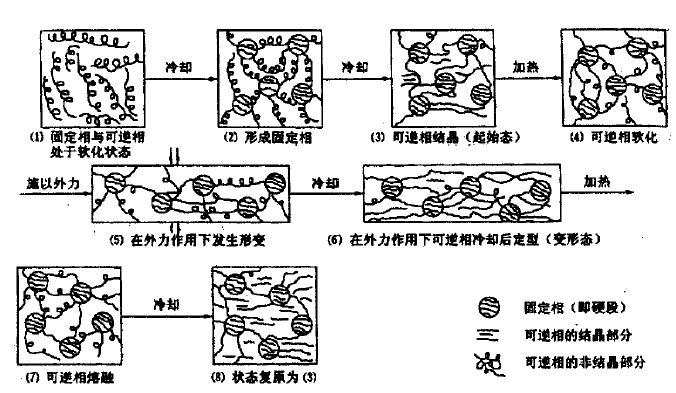
\includegraphics[width=0.75\textwidth]{figures/figure1}
 \caption{热塑性形状记忆聚氨酯的形状记忆机理示意图}\label{fig:diagram}
\end{figure}


\subsection{形状记忆聚氨酯的研究进展}
%\label{sec:requirements}
首例SMPU是日本Mitsubishi公司开发成功的……。

\subsection{水系聚氨酯及聚氨酯整理剂}

水系聚氨酯的形态对其流动性,成膜性及加工织物的性能有重要影响,一般分为三种类型\cite{Jiang2005Size} ,如表 \ref{tab:category}所示。

\begin{table}
  \centering
  \caption{水系聚氨酯分类} \label{tab:category}
  \begin{tabular*}{0.9\textwidth}{@{\extracolsep{\fill}}cccc}
  \toprule
    类别			&水溶型		&胶体分散型		&乳液型 \\
  \midrule
    状态			&溶解$\sim$胶束	&分散		&白浊 \\
    外观			&水溶型		&胶体分散型		&乳液型 \\
    粒径$/\mu m$	&$<0.001$		&$0.001-0.1$		&$>0.1$ \\
    重均分子量	&$1000\sim 10000$	&数千$\sim 20万$ &$>5000$ \\
  \bottomrule
  \end{tabular*}
\end{table}

\subsubsection{四级节标题}

根据需要,也可设四级节标题

由于它们对纤维织物的浸透性和亲和性不同,因此在纺织品染整加工中的用途也有差别,其中以水溶型和乳液型产品较为常用。另外,水系聚氨酯又有反应性和非反应性之分。虽然它们的共同特点是分子结构中不含异氰酸酯基,但前者是用封闭剂将异氰酸酯基暂时封闭,在纺织品整理时复出。相互交联反应形成三维网状结构而固着在织物表面。
……


%%
% The BIThesis Template for Graduate Thesis
%
% Copyright 2020-2022 Yang Yating, BITNP
%
% This work may be distributed and/or modified under the
% conditions of the LaTeX Project Public License, either version 1.3
% of this license or (at your option) any later version.
% The latest version of this license is in
%   http://www.latex-project.org/lppl.txt
% and version 1.3 or later is part of all distributions of LaTeX
% version 2005/12/01 or later.
%
% This work has the LPPL maintenance status `maintained'.
%
% The Current Maintainer of this work is Feng Kaiyu.
%
% Compile with: xelatex -> biber -> xelatex -> xelatex

\chapter{具体研究内容}

具体研究内容是学位论文的主要部分,是研究结果及其依据的具体表述,是研究能力的集中体现,一般应包括第2章、第3章至结论前一章。具体研究内容应该结构合理,层次清楚,重点突出,文字简练、通顺。可包括以下各方面:研究对象、研究方法、仪器设备、材料原料、实验和观测结果、理论推导、计算方法和编程原理、数据资料和经过加工整理的图表、理论分析、形成的论点和导出的结论等。具体研究内容各章后可有一节“本章小结”(必要时)。

\begin{theorem}[留数定理]
\label{thm:res}
  假设$U$是复平面上的一个单连通开子集,$a_1,\ldots,a_n$是复平面上有限个点,$f$是定义在$U\backslash \{a_1,\ldots,a_n\}$上的全纯函数,
  如果$\gamma$是一条把$a_1,\ldots,a_n$包围起来的可求长曲线,但不经过任何一个$a_k$,并且其起点与终点重合,那么:

  \begin{equation}
    \label{eq:res}
    \ointop_{\gamma}f(z)\,\mathrm{d}z = 2\pi\mathbf{i}\sum^n_{k=1}\mathrm{I}(\gamma,a_k)\mathrm{Res}(f,a_k)
  \end{equation}

  如果$\gamma$是若尔当曲线,那么$\mathrm{I}(\gamma, a_k)=1$,因此:

  \begin{equation}
    \label{eq:resthm}
    \ointop_{\gamma}f(z)\,\mathrm{d}z = 2\pi\mathbf{i}\sum^n_{k=1}\mathrm{Res}(f,a_k)
  \end{equation}

  在这里,$\mathrm{Res}(f, a_k)$表示$f$在点$a_k$的留数,$\mathrm{I}(\gamma,a_k)$表示$\gamma$关于点$a_k$的卷绕数。
  卷绕数是一个整数,它描述了曲线$\gamma$绕过点$a_k$的次数。如果$\gamma$依逆时针方向绕着$a_k$移动,卷绕数就是一个正数,
  如果$\gamma$根本不绕过$a_k$,卷绕数就是零。
\end{theorem}

\begin{proof}
  首先,由……

  其次,……

  所以……
  \qedhere
\end{proof}
  


\backmatter

%%==================================================
%% conclusion.tex for BIT Master Thesis
%% modified by yang yating
%% version: 0.1
%% last update: Dec 25th, 2016
%%==================================================


\begin{conclusion}

本文采用……。{\color{blue}(结论作为学位论文正文的最后部分单独排写,但不加章号。结论是对整个论文主要结果的总结。在结论中应明确指出本研究的创新点,对其应用前景和社会、经济价值等加以预测和评价,并指出今后进一步在本研究方向进行研究工作的展望与设想。结论部分的撰写应简明扼要,突出创新性。)}

\end{conclusion}
%%
% The BIThesis Template for Bachelor Graduation Thesis
%
% 北京理工大学毕业设计(论文)参考文献 —— 使用 XeLaTeX 编译
%
% Copyright 2020-2022 BITNP
%
% This work may be distributed and/or modified under the
% conditions of the LaTeX Project Public License, either version 1.3
% of this license or (at your option) any later version.
% The latest version of this license is in
%   http://www.latex-project.org/lppl.txt
% and version 1.3 or later is part of all distributions of LaTeX
% version 2005/12/01 or later.
%
% This work has the LPPL maintenance status `maintained'.
%
% The Current Maintainer of this work is Feng Kaiyu.
%
% Compile with: xelatex -> biber -> xelatex -> xelatex
%
% 如无特殊需要,本页面无需更改

% 参考文献开始
\chapter*{参考文献}
% 删除默认的「参考文献 / Reference」标题,使用上面定义的标题
\renewcommand{\thechapter}{参考文献}
% 添加到 TOC
\addcontentsline{toc}{chapter}{\thechapter}

% 设置参考文献字号为 5 号
\renewcommand*{\bibfont}{\zihao{5}}

% % 设置参考文献各个项目之间的垂直距离为 0
% \setlength{\bibitemsep}{1.1\itemsep}
\setlength{\bibnamesep}{0ex}
\setlength{\bibinitsep}{0ex}

% % 设置参考文献顺序标签 `[1]` 与文献内容 `作者. 文献标题...` 的间距
\setlength{\biblabelsep}{0.5mm}

% % 设置参考文献后文缩进为 0
\renewcommand{\itemcmd}{
  \addvspace{\bibitemsep} % 恢复 \bibitemsep 的作用
  \mkgbnumlabel{\printfield{labelnumber}}
  \hspace{\biblabelsep}}

\printbibliography[heading=none]


\begin{appendices}
\label{resources}
  \chapter{学习资料}

  \section{\LaTeX 学习资料推荐}
  \begin{itemize}[nosep]
    \item \href{https://www.overleaf.com/learn/latex/Tutorials}{《Overleaf 在线文档》(英文)} 提供了非常好的在线学习资源。
    \item \href{https://texdoc.org/serve/lshort-zh-cn.pdf/0}{《一份(不太)简短的 LATEX 2ε 介绍》} 可以作为更详尽的语法手册。
  \end{itemize}

  \section{\BIThesis 模板配置使用手册}
  \BIThesis{} 使用手册位于项目文件夹的 \verb|./bithesis.pdf|。它包括了关于 \BIThesis{} 的详细使用说明,
      对于每一个配置选项都有详细的说明和示例。
      
  \chapter{\BIThesis 与北理工历代\LaTeX{}模板项目简介}
  
\begin{itemize}[nosep]
  \item 在 2017 年之前,网络上已经出现一些北京理工大学学位论文 \LaTeX 模板。
    它们是“2012大眼小蚂蚁版”和“2016汪卫版”,均以上海交通大学的模板为基础。
  \item 2017 - 2018 年,计算机学院 2016 级研究生杨雅婷等人受研究生院委托,
    制作了\href{https://github.com/BIT-thesis/LaTeX-template}{BIT-Thesis} 
    研究生学位论文模板。
  \item 2019 - 2020 年,\BIThesis 最早由 2016 级的
    武上博、王赞、唐誉铭、牟思睿和詹熠莎等人维护。
    \begin{itemize}[nosep]
    \item 此时,\BIThesis 仅支持本科生毕业论文的排版。
    \item 在此期间,\BIThesis 从无到有诞生了,包括使用手册、
      在线文档和开箱即用的模板。
    \item 同时,2017 级的赵池等同学完成了一系列 \BIThesis 
      的视频教程。
    \item 武上博推进了教务部对 \BIThesis{} 的认可工作。
  \end{itemize}
  \item 2020 - 2021 年,2017 级的冯开宇、杨思云、郝正亮和顾骁等人
      接管了维护开发工作。
  \begin{itemize}[nosep]
    \item 在此期间,冯开宇将原来的 .tex 文件制作成了宏包,并发布到 CTAN 上。
    \item 此版本是 V2 版本,代号为 Birthday Cake.
  \end{itemize}
  \item 2021 - 2022 年,2021 级(硕士研究生)的冯开宇针对 2021、
      2022 毕业季收到的反馈对该项目进行维护升级。
  \begin{itemize}[nosep]
    \item 在此期间,冯开宇合入了杨雅婷等人在 2017 年开发的研究生学位论文模板。
    \item 次年暑假期间,冯开宇用 \verb|expl3| 重构了\LaTeX 样式代码,
      向用户提供了简易易用的接口。同时,也增加了本科全英文专业的毕设论文模板样式。
    \item 此版本是 V3 版本,代号为 Summer Time.
  \end{itemize}
  \item 2023 年,冯开宇在此版本上增加了多种新的功能,并修复了一些已知的问题。
  并推进了官方(教务部、研究生院)对 \BIThesis 的认可工作。
\end{itemize}

\end{appendices}

%%
% The BIThesis Template for experiment report
%
% Copyright 2020-2022 Yang Yating, BITNP
%
% This work may be distributed and/or modified under the
% conditions of the LaTeX Project Public License, either version 1.3
% of this license or (at your option) any later version.
% The latest version of this license is in
%   http://www.latex-project.org/lppl.txt
% and version 1.3 or later is part of all distributions of LaTeX
% version 2005/12/01 or later.
%
% This work has the LPPL maintenance status `maintained'.
%
% The Current Maintainer of this work is Feng Kaiyu.

% 1. 在 `./reference/pub.tex` 中添加数据。
% 2. 在 `./reference/pub.tex` 的数据中添加 `author+an` 字段表示你处于第几作者(参考示例)。
% 3. 在下方使用 `\nocite` 引用该文献(参考下方示例)。
% 4. 在下方使用 `\addtocategory` 将该文献添加至 `mypub` 类别(参考下方示例)。

\begin{publications}
  \nocite{myCiteKey}
  \nocite{myCiteKey2}
  \addtocategory{mypub}{myCiteKey}
  \addtocategory{mypub}{myCiteKey2}

  \printbibliography[heading=none,category=mypub,resetnumbers=true]{}
    % \item\textsc{高凌}. {交联型与线形水性聚氨酯的形状记忆性能比较}[J].
      % 化工进展, 2006, 532-535.(核心期刊)
    
\end{publications}

%%
% The BIThesis Template for experiment report
%
% Copyright 2020-2022 Yang Yating, BITNP
%
% This work may be distributed and/or modified under the
% conditions of the LaTeX Project Public License, either version 1.3
% of this license or (at your option) any later version.
% The latest version of this license is in
%   http://www.latex-project.org/lppl.txt
% and version 1.3 or later is part of all distributions of LaTeX
% version 2005/12/01 or later.
%
% This work has the LPPL maintenance status `maintained'.
%
% The Current Maintainer of this work is Feng Kaiyu.

\begin{acknowledgements}

本论文的工作是在导师……。

\textcolor{blue}{
  致谢是对下列方面致谢:资助和支持者;协助完成研究工作和提供便利条件者;在研究工作中提出建议和提供帮助者;给予转载和引用权的资料、图片、文献、研究思想和设想的所有者;其他应感谢者。致谢语言要诚恳、恰当、简短。
}

\end{acknowledgements}

%%==================================================
%% resume.tex for BIT Master Thesis
%% modified by yang yating
%% version: 0.1
%% last update: Dec 25th, 2016
%%==================================================

\begin{resume}

本人…。

\end{resume}


% 加入目录
\end{document}
